Komprimeringsalgoritmen "Huffman coding", er udviklet af David A. Huffman. Huffman udviklede algoritmen mens han var Ph.D studerende p� MIT. I 1952 udgav han dokumentet"A Method for the Construction of Minimum-Redundancy Codes"\cite{A_Method_for}. Her beskrev Huffman hvordan hans komprimerings algoritme fungerede. Hvad han havde udviklet, var en 'lossless' (tabsfri) komprimerings metode, hvilket betyder, at der ikke vil v�re noget tab af information ved at komprimere. Komprimeringsmetoden er beregnet til bin�re systemer, og form�let med algoritmen er at f� en given datam�nde til at benytte et minimalt antal bit. Dette kan opn�s ved at kigge p� hyppigheden af de forskellige tegn i datam�ngden der skal komprimeres, og give de oftest fremkommende symboler f� bits, og de mere sj�ldne symboler flere bits. Form�let er, at f� det gennemsnitlige antal bits pr. symbol ned. For s� at kunne f� de orginale data tilbage fra den komprimerede form, kr�ver det selvf�lgelig, at man har en form for ordbog, der beskriver hvilke tegn, der h�rer sammen med hvilke bits.

Dette princip kaldes entropikodning.



\begin{figure}[htb]
\centering
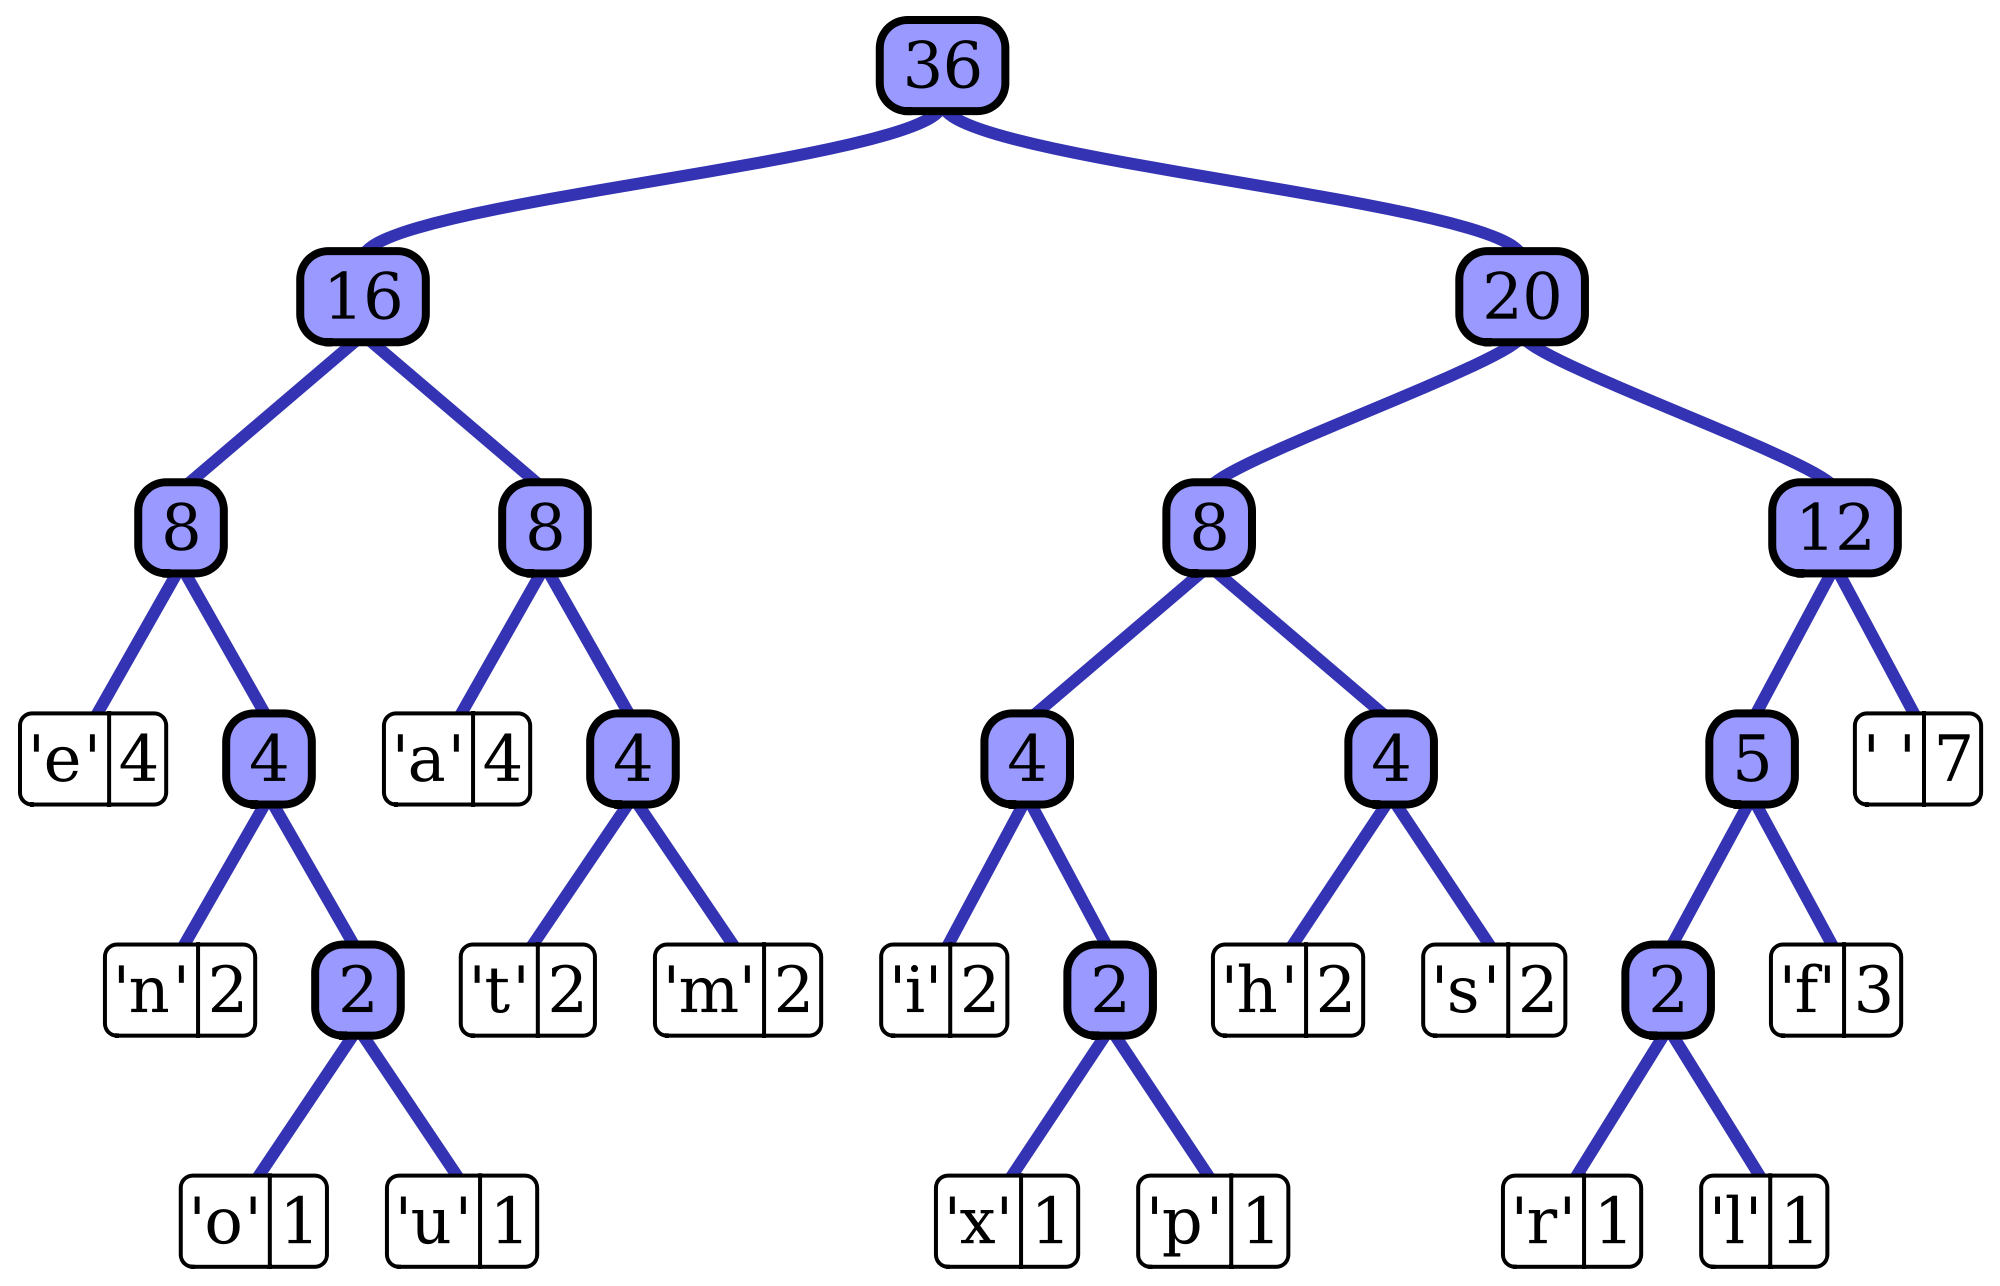
\includegraphics[scale=0.18]{Billeder/Huffman_tree_2.png}
\caption{Huffman tree}
%\label{fig:awesome_image}
\end{figure}